\subsection{La régression}

	\begin{frame}{Qu'est-ce qu'une régression?}
	La régression est une procédure statistique visant à établir la relation entre
	
		\begin{enumerate}
		    \item Une \textbf{variable d'intérêt}, également désignée comme variable réponse ou variable dépendante
		    
		    \item Une ou plusieurs \textbf{variables prédictives}, également désignées comme covariables, prédicteurs, ou variables indépendantes
		\end{enumerate}
	\end{frame}
	
	
	\begin{frame}{Qu'est-ce qu'une régression?}
	La régression est une procédure statistique visant à établir la relation entre
	
		\begin{enumerate}
		    \item Une \textbf{variable d'intérêt} $Y$ : vecteur d'observations de la réponse
		    
		    \item Une ou plusieurs \textbf{variables prédictives} $X$ :  vecteur ou matrice de prédicteurs pour chaque observation
		\end{enumerate}
		Le lien entre $X$ et $Y$ se fait au moyen d'une fonction $f$, estimée lors de la procédure de régression, telle que:
		\Large
		\begin{equation*}
		    Y_i = \textcolor{orange}{\textbf{f}}(X_i) + \epsilon_i
		\end{equation*}
		\small
		Avec $i$ allant de 1 à $N$, et $\epsilon_i$ l'erreur (ou résidus) du modèle, soit la variation de $Y$ non expliquée par les prédicteurs $X$.

	\end{frame}
	
	
	\begin{frame}{Exemple de régression : la biomasse}
	La régression est une procédure statistique visant à établir la relation entre
	
	
		\begin{enumerate}
		    \item Une \textbf{variable d'intérêt} $Y$ : la \textbf{biomasse} d'Arabidopsis thaliana 
		    
		    \centering 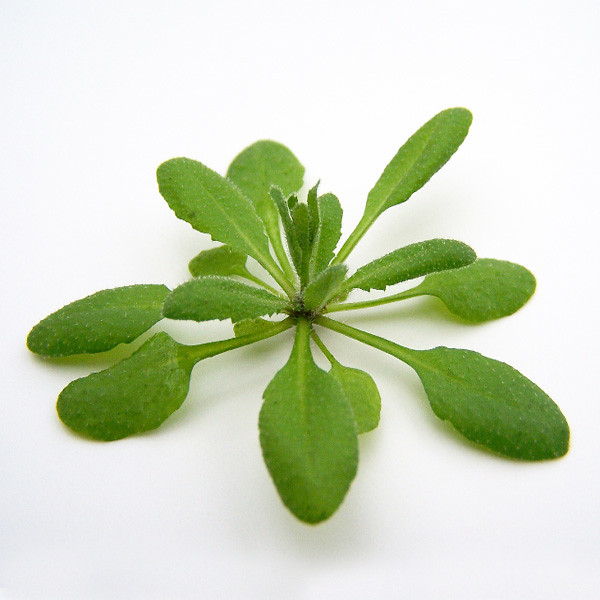
\includegraphics[scale = 0.041]{Figures/Intro/Arabidopsis.jpg}
		
		    
		    \item Une ou plusieurs \textbf{variables prédictives} $X$ :  \textbf{L'apport en nitrate, la température, l'humidité}, etc.
		\end{enumerate}
		
		
		\Large
		
		\begin{equation*}
		    Biomasse_i = \textcolor{orange}{\textbf{f}}(Nitrate_i) + \epsilon_i
		\end{equation*}
		
		\small
		Avec $i$ allant de 1 à $N$ correspondant à chacune des plantes du jeu de données, et $\epsilon_i$ la variation de biomasse non expliquée par l'apport en nitrate, la température, l'humidité, etc.

	\end{frame}
	
	
	\begin{frame}{Représentation graphique}
	Cas d'une régression \textbf{linéaire} à un prédicteur : $Y_i = \textcolor{orange}{\textbf{a}} + \textcolor{orange}{\textbf{b}}X_i + \epsilon_i$
	
	\vspace{0.5cm}
	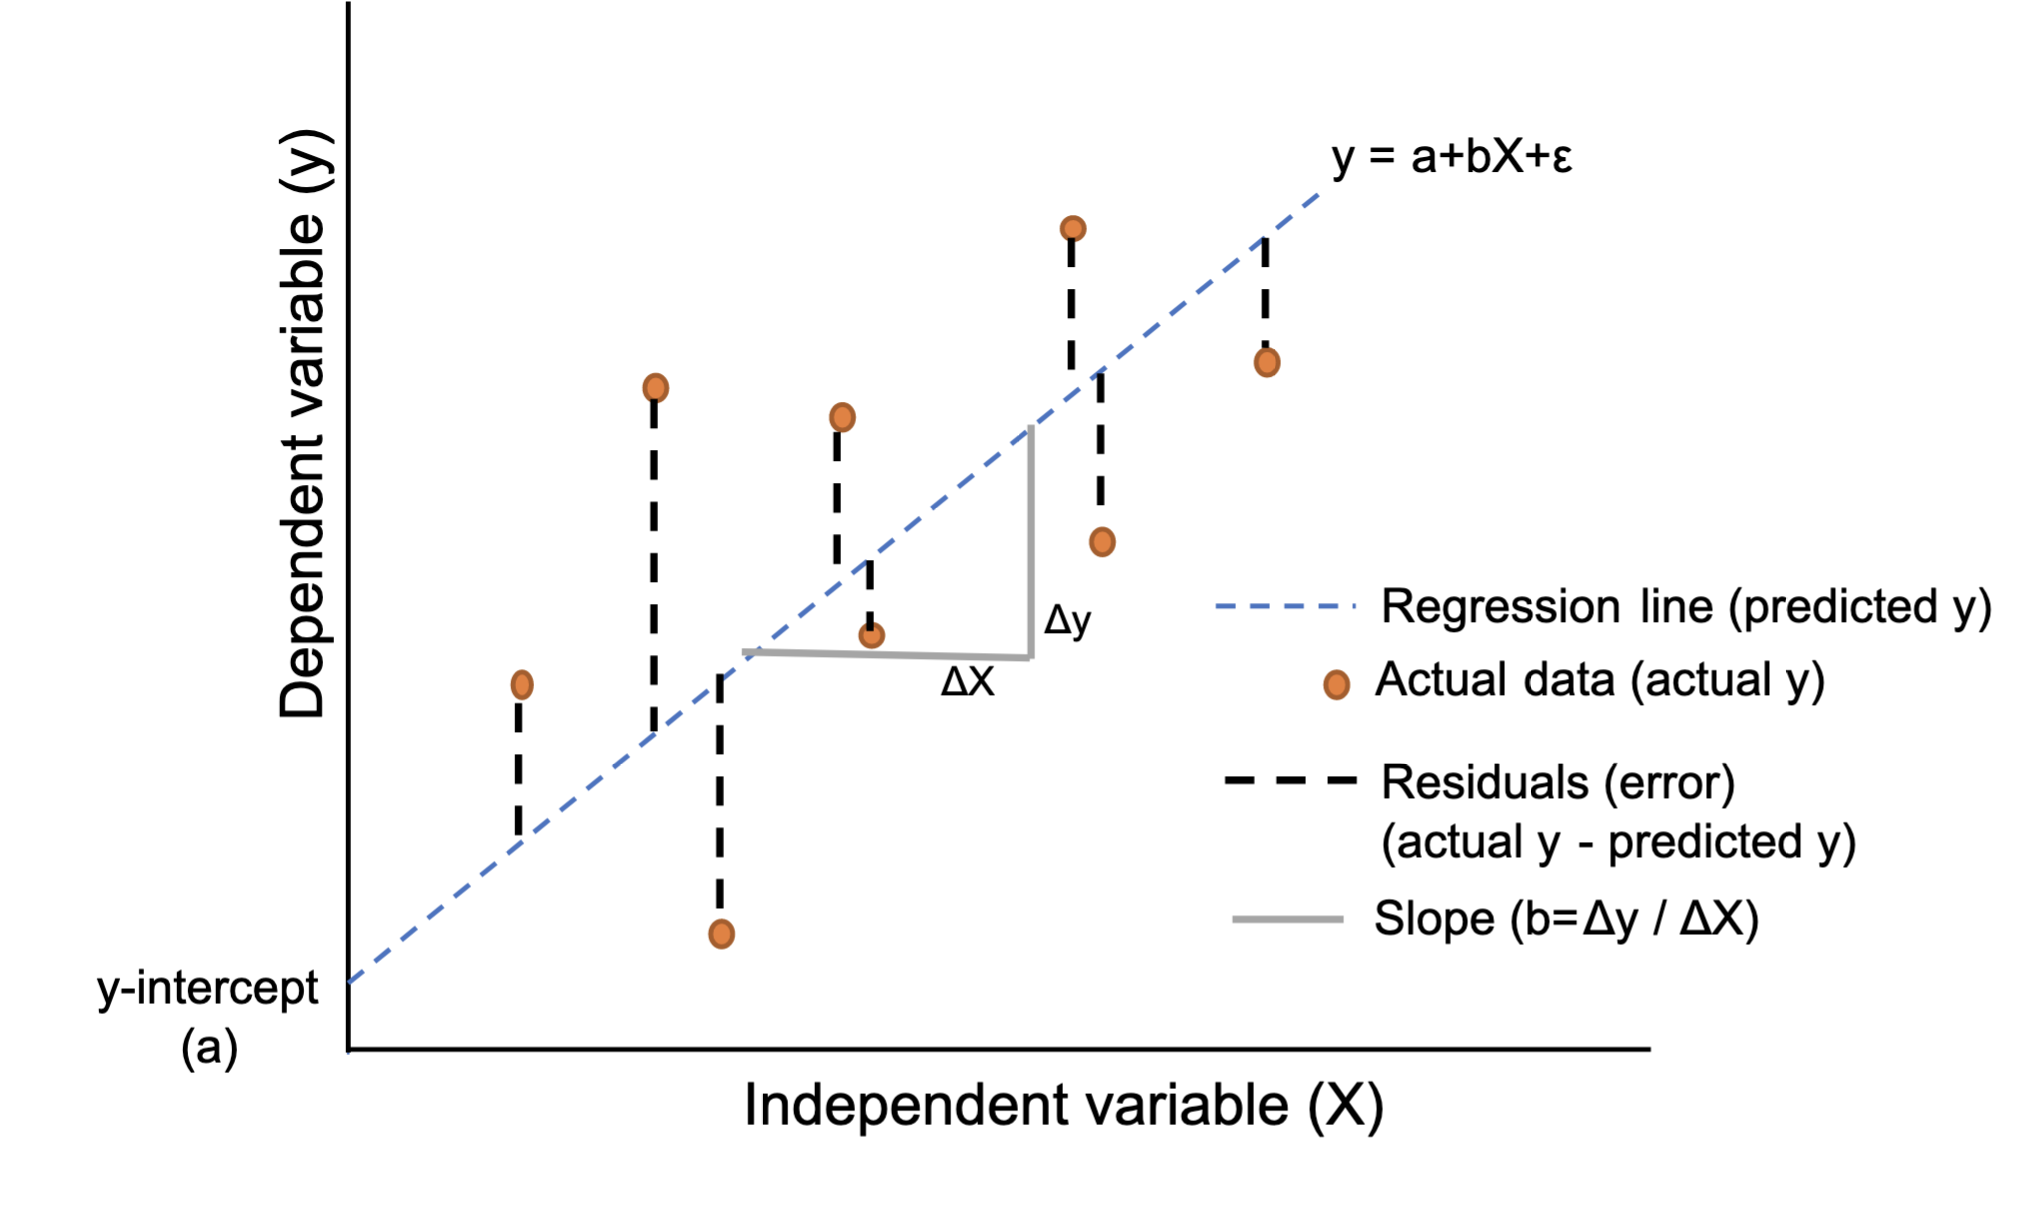
\includegraphics[scale=0.275]{Figures/Intro/regressionLine.png}
	\end{frame}
	
	
	\begin{frame}{Régression simple et régression multiple}
    	Cas d'une régression \textbf{linéaire} à deux prédicteurs (sans interaction): 
    	\begin{equation*}
    	    Biomasse_i = \textcolor{orange}{\textbf{a}} + \textcolor{orange}{\textbf{b}}Nitrate_i +\textcolor{orange}{\textbf{c}}Temperature_i + \epsilon_i
    	\end{equation*}
    	
    	\vspace{1cm}
    	\onslide<2> 
    	
    	Cas d'une régression \textbf{linéaire} à deux prédicteurs (avec interaction): 
    	\begin{equation*}
    	    Biomasse_i = \textcolor{orange}{\textbf{a}} + \textcolor{orange}{\textbf{b}}Nitrate_i +\textcolor{orange}{\textbf{c}}Temperature_i + \textcolor{orange}{\textbf{d}}Temperature_i*Nitrate_i + \epsilon_i
    	\end{equation*}
    	
    	
    	
	\end{frame}
	
	\begin{frame}{Remarques}

    	\textbf{Avantages de la régression : }
    	
    	
    	\begin{itemize} \scriptsize
    	\item Possibilité de prédire la variable d'intérêt pour un nouveau set de variables à l'outcome inconnu
    	    \item Quantification du pouvoir prédicteur de chaque variable d'entrée (ex: valeur du coefficient, et test sur la significativité de ce coefficient.)
    	\end{itemize}
    	
    	\onslide<2>
    	
    	
    	\vspace{0.5cm}
    	
    	\textbf{Extensions de la régression linéaire utiles à la suite du cours : }
    	
    	
    	
    	\begin{itemize} \scriptsize
    	
    	\item On peut ajouter des termes de pénalisation lors de l'estimation des coefficients afin de faire de la sélection de variables en grande dimension (lasso)
    	
    	\item La fonction $f$ n'est pas nécessairement une combinaison linéaire du type $\textcolor{orange}{\textbf{a}} + \textcolor{orange}{\textbf{b}}X1_i + \textcolor{orange}{\textbf{c}}X2_i$, mais peut prendre la forme des arbres de régression, des fonctions non linéaires plus adaptées à des questions biologiques complexes

    	\end{itemize}
    	
    	
	\end{frame}